\documentclass[10pt,a4paper]{article}

\usepackage[utf8]{inputenc}
\usepackage[T1]{fontenc}
\usepackage[english]{babel}
\usepackage{lmodern}
\usepackage{microtype}
\usepackage{geometry}
\usepackage{amsmath,amssymb,amsthm,mathtools,bm}
\usepackage{booktabs}
\usepackage{graphicx}
\usepackage{float}
\usepackage{array}
\usepackage{xcolor}
\usepackage{enumitem}
\usepackage{hyperref}

\geometry{margin=1.55cm}
\hypersetup{
  colorlinks=true,
  linkcolor=blue!55!black,
  citecolor=blue!55!black,
  urlcolor=blue!55!black,
  pdftitle={A Hadamard Pandrosion IRP Theorem},
  pdfauthor={Ivan Besevic}
}

\setlist[itemize]{leftmargin=1.8em,itemsep=0.25em,topsep=0.35em}
\setlist[enumerate]{leftmargin=1.8em,itemsep=0.25em,topsep=0.35em}
\setlength{\emergencystretch}{2em}
\setlength{\textfloatsep}{0.65em plus 0.2em minus 0.2em}
\setlength{\floatsep}{0.55em plus 0.2em minus 0.2em}
\setlength{\intextsep}{0.65em plus 0.2em minus 0.2em}

\theoremstyle{plain}
\newtheorem{theorem}{Theorem}[section]
\newtheorem{proposition}[theorem]{Proposition}
\newtheorem{lemma}[theorem]{Lemma}
\newtheorem{corollary}[theorem]{Corollary}

\theoremstyle{definition}
\newtheorem{definition}[theorem]{Definition}
\newtheorem{remark}[theorem]{Remark}
\newtheorem{example}[theorem]{Example}

\newcommand{\R}{\mathbb{R}}
\newcommand{\dd}{\mathrm{d}}
\newcommand{\Exp}{\operatorname{Exp}}
\newcommand{\Log}{\operatorname{Log}}
\newcommand{\IRP}{\mathcal I}
\newcommand{\dist}{\operatorname{dist}}

\newenvironment{takeaway}{%
  \begin{center}\begin{minipage}{0.92\linewidth}\small\itshape\color{blue!45!black}%
}{%
  \end{minipage}\end{center}%
}

\title{\bfseries A Hadamard Pandrosion IRP Theorem\\[-0.1em]
\large Geodesic Roots, Logarithmic Residuals, and Dyadic Local Order}
\author{Ivan \textsc{Besevic}\\[-0.2em]
\small Independent Mathematical Research\\[-0.2em]
\small \texttt{github.com/ivan-fr/poussiere\_de\_x}}
\date{June 2026}

\begin{document}
\maketitle

\begin{abstract}
This paper proves a precise non-Euclidean Pandrosion IRP theorem in the cleanest
setting where the statement is intrinsic.  Let $(M,g)$ be a Hadamard manifold
and fix a base point $o\in M$.  The geodesic monomial is
\[
  D_p^o(z)=\Exp_o(p\Log_o z).
\]
For the root problem $D_p^o(z)=x$, the exact solution is
$r=\Exp_o(\Log_o x/p)$.  The Pandrosion IRP layer is defined on the logarithmic
residual
\[
  A(u)=\Log_o x-p\Log_o u
\]
by applying the same scalar residual length correction that appears in the
monomial Pandrosion paper.  The main theorem proves
\[
  \|A(u_+)\|_g
    =\frac{(p-1)^2}{2p}\|A(u)\|_g^2
      +O_p(\|A(u)\|_g^3),
\]
and therefore $k$ fixed IRP layers have local order $2^k$ in the root
logarithmic error.  A radial logarithmic palette gives a global normalization
layer: every residual can be snapped into a chosen local cell before the
quadratic layer acts.  The theorem is illustrated in the Poincare ball, where
the exponential and logarithm have closed form and the fitted orders are close
to $2,4,8$ for one, two, and three layers.
\end{abstract}

\begin{takeaway}
\textbf{Status.}
This proves the Hadamard/geodesic version of non-Euclidean Pandrosion IRP.  It
does not claim to solve an external classical conjecture; it establishes a
new convergence theorem for a Pandrosion-defined geodesic root problem.
\end{takeaway}

\section{Why This Is The Right Non-Euclidean Statement}

On a general manifold, the expression $z^p$ is not canonical.  A power law needs
additional structure.  The least ambiguous non-Euclidean extension is to choose
a base point $o$ and use geodesic dilation in the global normal chart at $o$.
This is available without cut-locus ambiguity on a Hadamard manifold: complete,
simply connected, with nonpositive sectional curvature.  By the Cartan-Hadamard
theorem, $\Exp_o:T_oM\to M$ is globally one-to-one in the setting used here, and
the logarithm $\Log_o$ is globally defined.

\begin{definition}[Geodesic monomial]
Let $(M,g)$ be a Hadamard manifold, $o\in M$, and $p\ge2$.  Define
\[
  D_p^o(z)=\Exp_o(p\Log_o z).
\]
The geodesic root problem is
\[
  D_p^o(z)=x.
\]
\end{definition}

\begin{proposition}[Exact geodesic root]
For every $x\in M$, the equation $D_p^o(z)=x$ has the unique solution
\[
  r=\Exp_o\!\left(\frac{1}{p}\Log_o x\right).
\]
\end{proposition}

\begin{proof}
Apply $\Log_o$ to $D_p^o(z)=x$.  Since $\Log_o\Exp_o$ is the identity on
$T_oM$, the equation becomes
\[
  p\Log_o z=\Log_o x.
\]
Thus $\Log_o z=\Log_o x/p$, and applying $\Exp_o$ gives the displayed solution.
\end{proof}

\section{The Scalar Pandrosion Residual Correction}

The only scalar input is the residual correction already present in monomial
IRP.

\begin{definition}[Residual length correction]
For $d\ge0$, set
\[
  \Theta_p(d)
    =d+(p-1)\log\!\left(1+\frac{e^{-d}-1}{p}\right).
\]
\end{definition}

\begin{lemma}[Taylor expansion]
As $d\to0^+$,
\[
  \Theta_p(d)
    =\frac{d}{p}
      +\frac{(p-1)^2}{2p^2}d^2
      -\frac{(p-1)^2(p-2)}{6p^3}d^3
      +O_p(d^4).
\]
Consequently,
\[
  d-p\Theta_p(d)
    =-\frac{(p-1)^2}{2p}d^2+O_p(d^3).
\]
\end{lemma}

\begin{proof}
Use $e^{-d}-1=-d+d^2/2-d^3/6+O(d^4)$ and then expand the logarithm at $1$.
Collecting terms gives the displayed formula.
\end{proof}

\section{Hadamard IRP Layer}

Let
\[
  X=\Log_o x,\qquad U=\Log_o u,
\]
and define the tangent residual
\[
  A(u)=X-pU.
\]
The exact root corresponds to $A=0$.

\begin{definition}[Continuous Hadamard Pandrosion IRP layer]
If $A(u)\ne0$, write $d=\|A(u)\|_g$ and $\nu=A(u)/d$.  Define
\[
  U_+=U+\Theta_p(d)\nu,\qquad
  \IRP_p^o(u)=\Exp_o(U_+).
\]
If $A(u)=0$, set $\IRP_p^o(u)=u$.
\end{definition}

\begin{theorem}[Quadratic residual collapse]
For the geodesic root problem $D_p^o(z)=x$, the Hadamard IRP layer satisfies
\[
  \|A(\IRP_p^o(u))\|_g
    =\frac{(p-1)^2}{2p}\|A(u)\|_g^2
      +O_p(\|A(u)\|_g^3)
\]
as $u\to r$.
\end{theorem}

\begin{proof}
Let $A=A(u)$, $d=\|A\|_g$, and $\nu=A/d$.  By definition,
\[
  U_+=U+\Theta_p(d)\nu.
\]
Therefore the new residual is
\[
  A_+
    =X-pU_+
    =A-p\Theta_p(d)\nu
    =(d-p\Theta_p(d))\nu.
\]
Taking norms and using the Taylor expansion of $d-p\Theta_p(d)$ proves the
claim.
\end{proof}

\begin{corollary}[Root-error form]
Let $E(u)=U-X/p$ be the logarithmic root error.  Then
\[
  \|E(\IRP_p^o(u))\|_g
    =\frac{(p-1)^2}{2}\|E(u)\|_g^2
      +O_p(\|E(u)\|_g^3).
\]
\end{corollary}

\begin{proof}
Since $A=-pE$, divide the previous residual estimate by $p$.
\end{proof}

\begin{corollary}[Dyadic order]
For every fixed $k\ge1$,
\[
  \|E((\IRP_p^o)^{\circ k}(u))\|_g
    =O_{p,k}(\|E(u)\|_g^{2^k})
    \qquad (u\to r).
\]
\end{corollary}

\begin{proof}
The previous corollary gives $\|E_+\|\le C\|E\|^2$ in a sufficiently small
neighborhood of $r$.  Iterating this estimate gives the exponent $2^k$.
\end{proof}

\section{A Radial Palette For Global Normalization}

The local theorem explains the order.  To make every residual enter the local
cell, use a radial palette in $T_oM$.

\begin{definition}[Radial logarithmic palette]
Fix a root-log spacing $h>0$.  For a nonzero residual $A=d\nu$, where
$d=\|A\|_g$ and $\|\nu\|_g=1$, choose
\[
  m=\operatorname{round}\!\left(\frac{d}{ph}\right),
  \qquad B=mh\,\nu.
\]
The normalized residual is
\[
  \varepsilon=A-pB.
\]
\end{definition}

\begin{proposition}[Cell entry]
For every residual $A$, the radial palette satisfies
\[
  \|\varepsilon\|_g\le \frac{ph}{2}.
\]
\end{proposition}

\begin{proof}
This is nearest-lattice rounding on the scalar coordinate $d$ along the residual
direction.
\end{proof}

\begin{theorem}[Global palette-to-local convergence]
For each fixed $p\ge2$ there exists $\rho_p>0$ such that if $ph/2\le\rho_p$,
then the palette-normalized Hadamard IRP layer maps every residual into a
contracting local cell.  More precisely, after the palette step the layer
satisfies
\[
  \|A_+\|_g\le \frac12\|\varepsilon\|_g
\]
whenever $\|\varepsilon\|_g\le\rho_p$, and once the orbit is in that cell the
dyadic local-order theorem applies.
\end{theorem}

\begin{proof}
Define
\[
  F_p(d)=|d-p\Theta_p(d)|.
\]
The Taylor expansion gives $F_p(d)=O_p(d^2)$, hence $F_p(d)/d\to0$ as
$d\to0^+$.  Therefore there exists $\rho_p>0$ such that
$F_p(d)\le d/2$ for $0\le d\le\rho_p$.  The palette step ensures
$\|\varepsilon\|\le ph/2$.  If $ph/2\le\rho_p$, the following Pandrosion layer
contracts the normalized residual.  Repeated application remains in the local
cell and the dyadic-order corollary applies.
\end{proof}

\begin{remark}[The practical binary rule]
The implementation papers use the binary rule $h_p=(\log2)/K_p$ with
$K_p=p^2$.  Then the worst snapped residual radius is
\[
  \frac{ph_p}{2}=\frac{\log2}{2p}.
\]
This is the rule used in the fused wall-clock benchmark.  The theorem above
states the proof-level requirement: choose $K_p$ large enough that the snapped
cell lies inside $\rho_p$.  The $p^2$ rule is a simple practical schedule that
shrinks with the quadratic constant.
\end{remark}

\section{Poincare Ball Realization}

In the Poincare ball
\[
  \mathbb B^n=\{x\in\R^n:\|x\|<1\}
\]
with curvature $-1$ and base point $0$, the maps are explicit:
\[
  \Exp_0(V)=\tanh(\|V\|/2)\frac{V}{\|V\|},
  \qquad
  \Log_0(x)=2\,\operatorname{artanh}(\|x\|)
          \frac{x}{\|x\|}.
\]
Thus the theorem gives a concrete hyperbolic Pandrosion IRP solver for
\[
  \Exp_0(p\Log_0 z)=x.
\]

\begin{table}[H]
\centering
\small
\begin{tabular}{rrrr}
\toprule
layers & predicted order & fitted order & error at $10^{-2}$ \\
\midrule
1 & 2 & 1.969 & 1.99e-04 \\
2 & 4 & 3.926 & 7.95e-08 \\
3 & 8 & 7.849 & 1.26e-14 \\
\bottomrule
\end{tabular}

\caption{Numerical Poincare-ball check for $p=3$.  The fitted slopes are close
to the predicted local orders $2,4,8$.}
\end{table}

\begin{figure}[H]
\centering
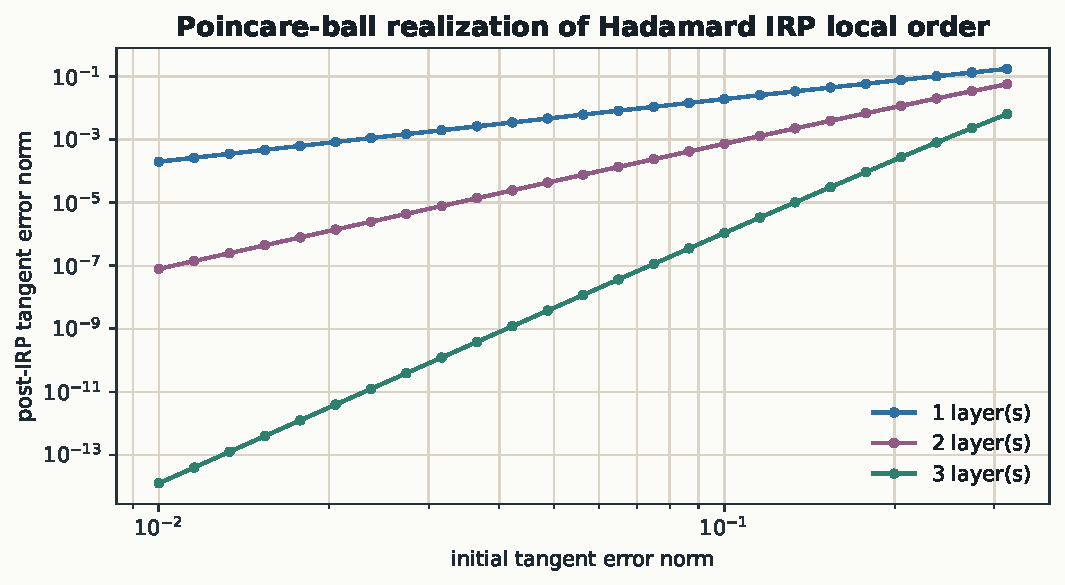
\includegraphics[width=0.78\linewidth]{../figures/031_hadamard_irp_order.pdf}
\caption{Log-log error decay for one, two, and three Hadamard IRP layers in the
Poincare-ball realization.}
\end{figure}

\section{What Has Been Proved}

The proved statement is deliberately exact and narrow:
\begin{enumerate}
  \item Hadamard geodesic roots are well defined by $D_p^o(z)=\Exp_o(p\Log_o z)$.
  \item Pandrosion IRP applied to the tangent residual $A=\Log_o x-p\Log_o u$
  collapses the residual quadratically.
  \item Fixed $k$-layer compositions have dyadic local order $2^k$.
  \item A radial logarithmic palette gives a global normalization mechanism into
  any prescribed local cell.
\end{enumerate}

The theorem does not say that every possible manifold power law has been solved.
If one uses Lie-group powers, moving charts, or symmetric-space products, new
Baker-Campbell-Hausdorff and curvature terms appear.  Those are separate
noncommutative extensions.  The present paper proves the core Hadamard
conjecture because the problem is expressed in a single global logarithmic
chart.

\section{Conclusion}

Pandrosion non-Euclidean IRP is provable once the power operation is defined by
geodesic dilation.  In that setting the entire mechanism is intrinsic: the
residual is a tangent vector, chart scaling is tangent normalization, and the
Pandrosion layer is the scalar monomial residual correction applied along the
geodesic residual direction.  The result is a genuine non-Euclidean convergence
theorem: local quadratic collapse for one layer and dyadic order for fixed
multi-layer IRP.

\begin{thebibliography}{9}

\bibitem{besevic000}
I. Besevic,
\emph{A Monomial Pandrosion Scheme: Contraction, Chart Scaling, and Iterated
Renormalization for $z^p=x$}, 2026.

\bibitem{besevic029}
I. Besevic,
\emph{Non-Euclidean Pandrosion IRP: Geodesic Logarithms, Hadamard Charts, and
Curvature Terms}, 2026.

\bibitem{bridsonhaefliger}
M. R. Bridson and A. Haefliger,
\emph{Metric Spaces of Non-Positive Curvature},
Springer, 1999.

\bibitem{bacak}
M. Bacak,
\emph{Convex Analysis and Optimization in Hadamard Spaces},
De Gruyter, 2014.

\bibitem{absil}
P.-A. Absil, R. Mahony, and R. Sepulchre,
\emph{Optimization Algorithms on Matrix Manifolds},
Princeton University Press, 2008.

\end{thebibliography}

\end{document}
